\documentclass[conference]{IEEEtran}
\IEEEoverridecommandlockouts
% The preceding line is only needed to identify funding in the first footnote. If that is unneeded, please comment it out.
\usepackage{cite}
\usepackage{amsmath,amssymb,amsfonts}
\usepackage{algorithmic}
\usepackage{graphicx}
\usepackage{textcomp}
\def\BibTeX{{\rm B\kern-.05em{\sc i\kern-.025em b}\kern-.08em
    T\kern-.1667em\lower.7ex\hbox{E}\kern-.125emX}}
\usepackage[utf8]{inputenc}
\usepackage[spanish]{babel}
\usepackage[table,xcdraw]{xcolor} % Tablas

\usepackage{minted}

\usepackage{cuted}

\usepackage{url}

\usepackage{listings} % Código

\lstset{literate=
  {á}{{\'a}}1 {é}{{\'e}}1 {í}{{\'i}}1 {ó}{{\'o}}1 {ú}{{\'u}}1
  {Á}{{\'A}}1 {É}{{\'E}}1 {Í}{{\'I}}1 {Ó}{{\'O}}1 {Ú}{{\'U}}1
  {à}{{\`a}}1 {è}{{\`e}}1 {ì}{{\`i}}1 {ò}{{\`o}}1 {ù}{{\`u}}1
  {À}{{\`A}}1 {È}{{\'E}}1 {Ì}{{\`I}}1 {Ò}{{\`O}}1 {Ù}{{\`U}}1
  {ä}{{\"a}}1 {ë}{{\"e}}1 {ï}{{\"i}}1 {ö}{{\"o}}1 {ü}{{\"u}}1
  {Ä}{{\"A}}1 {Ë}{{\"E}}1 {Ï}{{\"I}}1 {Ö}{{\"O}}1 {Ü}{{\"U}}1
  {â}{{\^a}}1 {ê}{{\^e}}1 {î}{{\^i}}1 {ô}{{\^o}}1 {û}{{\^u}}1
  {Â}{{\^A}}1 {Ê}{{\^E}}1 {Î}{{\^I}}1 {Ô}{{\^O}}1 {Û}{{\^U}}1
  {Ã}{{\~A}}1 {ã}{{\~a}}1 {Õ}{{\~O}}1 {õ}{{\~o}}1
  {œ}{{\oe}}1 {Œ}{{\OE}}1 {æ}{{\ae}}1 {Æ}{{\AE}}1 {ß}{{\ss}}1
  {ű}{{\H{u}}}1 {Ű}{{\H{U}}}1 {ő}{{\H{o}}}1 {Ő}{{\H{O}}}1
  {ç}{{\c c}}1 {Ç}{{\c C}}1 {ø}{{\o}}1 {å}{{\r a}}1 {Å}{{\r A}}1
  {€}{{\euro}}1 {£}{{\pounds}}1 {«}{{\guillemotleft}}1
  {»}{{\guillemotright}}1 {ñ}{{\~n}}1 {Ñ}{{\~N}}1 {¿}{{?`}}1
}

\definecolor{mGreen}{rgb}{0,0.6,0}
\definecolor{mGray}{rgb}{0.5,0.5,0.5}
\definecolor{mPurple}{rgb}{0.58,0,0.82}
\definecolor{backgroundColour}{rgb}{0.95,0.95,0.92}

\lstdefinestyle{CStyle}{
    backgroundcolor=\color{backgroundColour},   
    commentstyle=\color{mGreen},
    keywordstyle=\color{magenta},
    numberstyle=\tiny\color{mGray},
    stringstyle=\color{mPurple},
    basicstyle=\footnotesize,
    breakatwhitespace=false,         
    breaklines=true,                 
    captionpos=b,                    
    keepspaces=true,                 
    numbers=left,                    
    numbersep=5pt,                  
    showspaces=false,                
    showstringspaces=false,
    showtabs=false,                  
    tabsize=2,
    language=C
}

\lstdefinestyle{customasm}{
  backgroundcolor=\color{backgroundColour},   
    %commentstyle=\color{mGreen},
    keywordstyle=\color{magenta},
    numberstyle=\tiny\color{mGray},
    stringstyle=\color{mPurple},
    basicstyle=\footnotesize,
    breakatwhitespace=false,         
    breaklines=true,                 
    captionpos=b,                    
    keepspaces=true,                 
    numbers=left,                    
    numbersep=5pt,                  
    showspaces=false,                
    showstringspaces=false,
    showtabs=false,                  
    tabsize=2,
  language=[x86masm]Assembler
}

\begin{document}

\def\UrlBreaks{\do\/\do-\do\_} % Para que las URLs no sobrepasen (generalmente) una columna en longitud

\title{Estudio del efecto del principio de localidad en el acceso a datos en programas\\
%{\footnotesize \textsuperscript{*}Note: Sub-titles are not captured in Xplore and
%should not be used}
%\thanks{Identify applicable funding agency here. If none, delete this.}
}

\author{\IEEEauthorblockN{Álvaro Goldar Dieste}
\IEEEauthorblockA{\textit{Universidad de Santiago de Compostela} \\
%%\textit{name of organization (of Aff.)}\\
Santiago de Compostela, España \\
alvaro.goldar@rai.usc.es}
\and
\IEEEauthorblockN{Francisco Javier Cardama Santiago}
\IEEEauthorblockA{\textit{Universidad de Santiago de Compostela} \\
%\textit{name of organization (of Aff.)}\\
Santiago de Compostela, España \\
franciscojavier.cardama@rai.usc.es}
}

\maketitle

% Insertar tras maketitle para mostrar los números de página
\thispagestyle{plain}
\pagestyle{plain}

\begin{abstract}
En este documento se estudia el efecto del principio de localidad en el acceso a datos en programas, empleando un computador específico. 

Se parte de un código inicial, con el que se realizan diversas pruebas con las que estudiar el número de ciclos medios por acceso a memoria y, posteriormente, el efecto de las precargas por \textit{software} y \textit{hardware} en la caché. Estas pruebas se basan en la reducción de una suma en punto flotante de doble precisión de un subconjunto de los elementos de un array \textit{A[]} equiespaciados en \textit{D}, distribuidos a lo largo de \textit{L} líneas caché. Estos parámetros se irán variando para analizar cómo afectan al rendimiento del programa.

Mediante estas pruebas se termina por concluir que el rendimiento del programa es menor a medida que la separación entre los elementos del array \textit{A[]} y el tamaño del experimento crecen; por otra parte, el empleo de la precarga parece mejorar levemente el rendimiento global.

\textbf{\textit{Palabras clave}---caché, jerarquía de memoria, latencia, principio de localidad, precarga}
\end{abstract}

%\begin{IEEEkeywords}
%component, formatting, style, styling, insert
%\end{IEEEkeywords}

\section{Introducción}
En cada uno de los experimentos llevados a cabo se determina el coste temporal de un bucle de computación, el cual precisa leer constantemente datos dispuestos en memoria, estimándose así el número medio de ciclos del procesador por acceso a memoria. Estos experimentos son llevados a cabo en un computador en específico, cuyas especificaciones de interés se encuentran descritas en la sección \ref{descripcionComputador}.

A continuación, se analiza el tipo de experimento a realizar en la sección \ref{tipoExperimento}. Para ello, se ha elaborado un programa de pruebas en el lenguaje C, en el cual se variarán los parámetros de entrada disponibles en cuanto al patrón de accesos a realizar y el tamaño del conjunto de datos a procesar. Además, también se comprueban, en la sección \ref{tipoPrecargas}, las técnicas de precarga disponibles en el computador de pruebas y cómo se analizarán sus efectos.

Con ello, conociendo ya la arquitectura de la memoria caché dispuesta en el procesador escogido, se realizarán y analizarán todas las pruebas en la sección \ref{experimentos}, siendo posible determinar los efectos del principio de localidad y de la precarga de datos (\textit{prefetching}) sobre el programa en función de los ciclos medios por acceso obtenidos y los valores dados como parámetros de entrada.

Finalmente, se tratan, a modo de resumen, las conclusiones extraídas a partir de las pruebas realizadas en la sección \ref{resumenExperimentos}.

\section{Computador empleado en los experimentos} \label{descripcionComputador}

\subsection{Jerarquía de memoria del procesador}
El modelo de procesador escogido para la realización de las pruebas es el Intel Core i3-7100 \cite{procesador}. Este tiene la capacidad de ejecutar hasta cuatro hilos simultáneamente, pero al centrarse el objetivo de los experimentos en los efectos sobre una única jerarquía de memoria caché, tan solo se considerará un único núcleo del procesador para ello, y por ende el programa de pruebas se ejecutará sobre un único hilo.

Un núcleo del procesador cuenta con un total de cuatro cachés: dos cachés L1, una caché L2, y una caché L3. Las cachés L1 son, respectivamente, de instrucciones y de datos, por lo cual tan solo será de interés esta última al estudiarse los efectos sobre los datos. Por otra parte, los niveles L2 y L3 son compartidos entre instrucciones y datos, pero no supondrá un inconveniente para los experimentos dado que se realizarán constantemente las mismas operaciones, al estudiarse un bucle computacional de poca extensión.

Los datos de las tres memorias caché de interés se ven reflejados en el Cuadro \ref{especificacionesCaches}.

\begin{table}[htbp]
\caption{Especificaciones de las cachés de interés de la CPU.}
\begin{center}
\begin{tabular}{|c|c|c|c|c|}
\hline
\rowcolor[HTML]{EFEFEF} 
\textbf{CACHÉ}                                  & \textbf{Tamaño} & \textbf{Vías} & \textbf{Conjuntos} & \textbf{Tamaño conjunto} \\ \hline
\cellcolor[HTML]{EFEFEF}\textbf{L1 (datos)}      & 32 KB           & 8             & 64                 & 512 bytes                \\ \hline
\cellcolor[HTML]{EFEFEF}\textbf{L2 (unificada)} & 256 KB          & 4             & 1024               & 256 bytes                \\ \hline
\cellcolor[HTML]{EFEFEF}\textbf{L3 (unificada)} & 3072 KB         & 12            & 4096               & 768 bytes                \\ \hline
\end{tabular}
\label{especificacionesCaches}
\end{center}
\end{table}

\subsection{Sistema Operativo}

Los experimentos se ejecutarán sobre el sistema operativo GNU/Linux, concretamente sobre la distribución Ubuntu 16.04.5 LTS basada en Debian, empleando la versión 4.4.0-131-generic del respectivo kernel.

Se procurará reducir al mínimo los programas en ejecución durante los experimentos para que no interfieran con el programa de pruebas. Además, es conveniente que una ejecución de este último suponga un único experimento, para reducir también la posibilidad de que el planificador del sistema operativo interfiera en las pruebas.

Para este último aspecto, se ha elaborado un script en el lenguaje Python mediante el cual automatizar las pruebas a realizar, relegando a este la tarea de variar los parámetros de entrada del programa en C para ejecutarlo un número determinado de veces, y de generar tras ello las gráficas de los experimentos realizados.

\section{Programa de pruebas} \label{tipoExperimento}

\subsection{Funcionamiento del programa}
El programa realiza una reserva de memoria para un número determinado de elementos de tipo \texttt{Double}, tras lo cual accede tan solo a un subconjunto de ellos, todo ello en función de los parámetros de entrada, efectuando una reducción de punto flotante sobre estos últimos. Es en esta sección del programa en donde se encuentra el bucle computacional de interés, y se ejecuta un total de 10 veces.

El programa requiere los siguientes valores para su ejecución:
\begin{itemize}
\item \textbf{\textit{A[]}}: array de elementos \texttt{Double} reservados.
\item \textbf{\textit{D}}: paso entre los valores a los que acceder.
\item \textbf{\textit{L}}: número de líneas caché L1 a las que acceder, existiendo siete valores que probar con cada \textit{D}, y calculadas en función de \textit{S1} y \textit{S2}.
\item \textbf{\textit{S1}}: número de líneas que caben en la caché L1 de datos.
\item \textbf{\textit{S2}}: número de líneas que caben en la caché L2.
\item \textbf{\textit{R}}: número de elementos de \textit{A[]} a los que acceder, en función del paso \textit{D} y de modo que se acceda a las \textit{L} líneas diferentes.
\item \textbf{\textit{e[]}}: array con los índices de los elementos de \textit{A[]} a los que acceder, puesto que el acceso a los elementos de \textit{A[]} no se realiza de forma directa.
\end{itemize}

Consecuentemente, puede concretarse la reducción de punto flotante mediante la siguiente expresión:
\begin{equation*}
	    A[0] + A[D] + A[2D] + ... + A[(R-1)\cdot D] = \sum_{i=0}^{R-1}A[i\cdot D].
\end{equation*}

Cabe además destacar que es conveniente alinear la reserva de memoria al inicio de una línea caché, para lo cual se dispone de la función \texttt{\_mm\_malloc(TC,CLS)}, siendo \textit{TC} el número de bytes a reservar y \textit{CLS} el tamaño de una línea caché en bytes. Esta función devuelve un puntero alineado a \textit{CLS} bytes.

También se incluye una fase de calentamiento mediante la cual evitar efectos de inicialización de componentes como las cachés o las TLBs. Esta simplemente consiste en inicializar los valores del vector \textit{A[]} a emplear.

\subsection{Cálculo de \textit{R}}
Para obtener el valor apropiado de \textit{R} en función de el valor \textit{D} dado y el \textit{L} correspondiente, es necesario diferenciar dos escenarios.

En el caso de que el paso especificado no supere el tamaño de una línea, se debe reservar memoria para, a lo sumo, \textit{L} líneas consecutivas. Se calcula entonces el número de elementos a leer \textit{R} en función de cuántos caben en las \textit{L} líneas, y dividiendo en función del paso.

Sin embargo, si el paso especificado supera el tamaño de una línea, es altamente probable que en algún momento durante la ejecución se salte una de las líneas reservadas a causa del paso y, de este modo, el cálculo de \textit{R} no resultaría en las \textit{L} líneas diferentes que se deben leer.

Para ello, simplemente es necesario asignar a \textit{R} el número de líneas caché distintas a leer puesto que, al disponer de un paso mayor al tamaño de una línea, en ningún momento se leen dos valores pertenecientes a la misma línea caché.

\subsection{Cálculo de \textit{TC}}
Para obtener el tamaño necesario para la reserva de elementos del array \textit{A[]}, es necesario considerar tanto el número de elementos a leer en memoria como el paso entre estos.

Por lo tanto, al ser $R_{0}$ el primer elemento de \textit{A[]}, es necesario reservar memoria para un elemento y, para cada uno de los restantes elementos a leer, reservar \textit{D} elementos para respetar el paso dado.

\subsection{Código fuente}
Se dispone a continuación el código fuente del programa de pruebas escrito en C para los experimentos. Empleando el compilador \textit{GCC} en su versión 5.4.0, es importante especificar la opción \texttt{-O0} para que no se efectúe ningún tipo de optimización en el código puesto que, en caso contrario, el compilador podría decidir eliminar el bucle computacional si detectase que los resultados nunca serían empleados.

De todos modos, antes de finalizar la ejecución se imprimen los resultados de los cómputos realizados, evitando de este modo a la fuerza que el compilador pueda efectuar la optimización descrita anteriormente.

\begin{lstlisting}[style=CStyle, title=Programa de pruebas en C.]
#include <stdio.h>
#include <stdlib.h>
#include <math.h>
#include <pmmintrin.h>
#include <time.h>
#include <unistd.h>

/* Especificaciones de la CPU */
#define S1 64 * 8
#define S2 1024 * 4
#define CLS 64

/* Macros auxiliares */
#define NUM_S 10
#define DOUBLES_LINEA CLS / sizeof( double )

/* Funciones a emplear */
void start_counter();
double get_counter();
double mhz();

/* Se inicializa el contador de ciclos */
static unsigned cyc_hi = 0;
static unsigned cyc_lo = 0;

/* Main */
int main(int argc, char **argv)
{
  /* Variables a emplear */
  double ck;
  // Valor D
  int D;
  // Valores L
  int valoresL[] = { S1 / 2, 3 * S1 / 2, S2 / 2, 3 * S2 / 4, 2 * S2, 4 * S2, 8 * S2 };
  // Valor R
  int R;
  // Valores e
  int *e;
  // Valores S
  double valoresS[ NUM_S ];
  // Valores A
  double *valoresA;
  // TC calculado
  int TC;
  // Suma temporal
  double suma;
  // Contadores
  int i;
  int j;
  // Fichero en el que guardar el resultado
  FILE *fichero;

  /***** Argumentos *****/

  if( argc < 3 )
  {
    printf( "Número de valores incorrecto. Uso: % s   <D> <L>", argv[ 0 ] );
    exit( EXIT_FAILURE );
  }

  /***** Inicialización *****/

  // Semilla para generar números aleatorios
  srand( ( unsigned )time( NULL ) );

  // Valor de D obtenido de los argumentos
  D = atoi( argv[ 1 ] );

  // Valor para R en función del D obtenido
  if( D <= DOUBLES_LINEA )
  {
      R = ( int )ceil( valoresL[ atoi( argv[ 2 ] ) ]    * DOUBLES_LINEA / D );
  }
  else
  {
      R = valoresL[ atoi( argv[ 2 ] ) ];
  }

  // Valores para e, reservando en primer lugar
  // espacio para las posiciones pertinentes
  if( ( e = ( int * )malloc( R * sizeof( int ) ) )  == NULL )
  {
      perror( "Reserva de memoria fallida" );
      exit( EXIT_FAILURE );
  }

  // El límite superior es el número de valores con
  // los que efectuar la suma
  for( i = 0; i < R; i++ )
  {
    // Se consideran el número de posición y el paso
    // dado
    e[ i ] = i * D;
  }

  // Se obtienen valores para A, reservando memoria
  // para los elementos intermedios
  TC = ( R - 1 ) * D + 1;

  // Se alinea la reserva al inicio de una línea de
  // la caché
  if( ( valoresA = _mm_malloc( TC * sizeof( double ), CLS ) ) == NULL )
  {
      perror( "Reserva de memoria fallida" );
      exit( EXIT_FAILURE );
  }

  // Se genera en cada posición un valor entre 1 y
  // 2 (positivo o negativo)
  for( i = 0; i < TC; i++ )
  {
      valoresA[ i ] = ( ( double )rand() / RAND_MAX     + 1 ) * pow( -1, rand() % 2 );
  }

  /***** Pruebas *****/

  // Se registra el contador de la CPU
  start_counter();

  // Se realizan las sumas especificadas
  for( i = 0; i < NUM_S; i++ )
  {
      // Se emplean los índices calculados
      for( j = 0, suma = 0; j < R; j++ )
      {
          // Se realiza el acceso a memoria
          suma += valoresA[ e[ j ] ];
      }

      // Se almacena la reducción de punto flotante
      valoresS[ i ] = suma;
  }

  // Se registran los ciclos transcurridos desde el
  // registro del contador
  ck = get_counter();

  // Se abre el fichero
  if( ( fichero = fopen( "resultado.csv", "a" ) ) == NULL )
  {
      perror( "No se ha podido abrir el fichero para    escritura" );
      exit( EXIT_FAILURE );
  }

  // Se guardan el valor de L, el número de ciclos
  // medios por acceso y el valor de D en un formato
  // csv que vaya a interpretar el graficador
  fprintf( fichero, "% d,%1.10lf,%d\n", valoresL[ atoi( argv[ 2 ] ) ],
    ck / ( NUM_S * R ), D );

  // Se imprimen las sumas realizadas
  for( i = 0; i < NUM_S; i++ )
  {
      printf( "% f\n", valoresS[ i ] );
  }
  
  // Se libera la memoria reservada
  free( e );
  _mm_free( valoresA );

  return( EXIT_SUCCESS );
}
\end{lstlisting}

\section{Efectos de la precarga sobre los experimentos} \label{tipoPrecargas}

\subsection{La precarga en el procesador de pruebas}

Existe una técnica para incrementar la velocidad de ejecución de un código, denominada \textit{precarga (prefetching)}. Esta consiste en cargar datos, bien sean instrucciones o no, antes de que el procesador los necesite, trayéndolos de la zona de la jerarquía de memoria en donde se encuentren a una zona que esté más cercana al procesador.

Intel, el fabricante del procesador de pruebas, ofrece dos implementaciones de la precarga: mediante hardware y mediante software \cite{precargas}.

Empleando el hardware, el procesador se encarga de identificar patrones de acceso a datos para traer datos a la memoria caché.

Por otra parte, el procesador cuenta, en su repertorio de instrucciones, con órdenes que permiten a un programa precargar un dato especificado en el nivel de la caché indicado. Normalmente, es el propio compilador el que se encarga de introducir estas instrucciones en los lugares y situaciones apropiados a la hora de generar el código en ensamblador de un programa.

Sin embargo, esta característica debe ser empleada con precaución, puesto que un mal uso puede derivar en una pérdida de eficiencia. Por ejemplo, la precarga de un dato que no será referenciado supondrá una carga extra e innecesaria para el procesador, además de que estará ocupando parte del valioso espacio disponible en la memoria caché.

Consecuentemente, es habitual que un compilador permita decidir al usuario si realizar este tipo de optimización o no. En este caso, el compilador \textit{GCC} empleado permite activar o desactivar esta característica a la hora de iterrar sobre arrays empleando las opciones \texttt{-fprefetch-loop-arrays} y \texttt{-fno-prefetch-loop-arrays} respectivamente.

\subsection{Experimentos adicionales estudiando la precarga}

Para observar en qué medida puede beneficiar o perjudicar la técnica de la precarga a un programa basado fundamentalmente en el acceso a datos, como es el caso del programa de pruebas de los experimentos a realizar, se efectuarán a mayores una serie de experimentos en los que se intentará estudiar su influencia.

En primer lugar, se compararán los resultados obtenidos del programa en una compilación sin precarga mediante software frente a una versión que sí será optimizada por el compilador.

Continuando, dado que no es posible deshabilitar la precarga por hardware que el procesador trata de realizar identificando patrones, se tratará de dificultarle esta tarea alterando la generación de índices del array \textit{e[]}. La modificación consistirá en añadir a cada índice un valor entero en el rango $[0, 3]$, de modo que los datos accedidos no se encuentren equitativamente espaciados.

\section{Realización de los experimentos} \label{experimentos}

\subsection{Automatización de los experimentos}
Tal y como se ha mencionado previamente, la realización de los experimentos se ha apoyado en un script en el lenguaje Python. Este se encarga de, a partir de cinco valores para \textit{D} dados, ejecutar el programa de pruebas con cada uno de ellos y con los siete valores de \textit{L} posibles.

Todo ello se ejecuta un total de 10 veces, con el objetivo de considerar la posible variabilidad de los resultados entre ejecuciones.

\subsection{Resultados de los experimentos}
Para los valores de \textit{D} es de importancia escoger un conjunto que permita observar los efectos del principio de localidad sobre los experimentos. Por ejemplo, escoger cinco valores consecutivos no sería de utilidad porque, muy probablemente, los resultados serían muy similares.

Los experimentos se han realizado por lo tanto sobre los siguientes valores de \textit{D}: 1, 12, 38, 64 y 72.

Es necesario tener presentes las siguientes variantes a la hora de interpretar los resultados de los experimentos:
\begin{itemize}
    \item \textbf{\textit{D}}: determina cómo de distanciados se encuentran los valores a referenciar; consecuentemente, un mayor paso implica un menor cumplimiento del principio de localidad.
    \item \textbf{\textit{L}}: determina el número de líneas distintas a las que es necesario acceder; un mayor número de líneas implica que se vean potenciados los efectos provocados por el resto de parámetros, al incrementar la extensión del experimento.
    \item Como consecuencia, \textit{D} y \textit{L} condicionan el número de líneas sin referenciar en un experimento; debe tenerse presente esto puesto que, al inicializarse todos los valores del array \textit{A[]} antes del bucle computacional, será posible encontrar en las memorias caché una cantidad relevante de líneas que no se referenciarán en el bucle computacional, cumpliéndose en menor medida el principio de localidad.
\end{itemize}

En la Figura \ref{valoresD} se pueden observar los resultados de los experimentos en función del valor dado para \textit{D}. Se representan el promedio y la mediana para los ciclos obtenidos en cada conjunto de experimentos de cada \textit{D}: la mediana se emplea para representar un valor global del resultado evitando que los extremos lo condicionen, y el promedio se muestra para ver en qué medida estos valores dispares afectan al valor global.

\begin{figure}[htbp]
\centerline{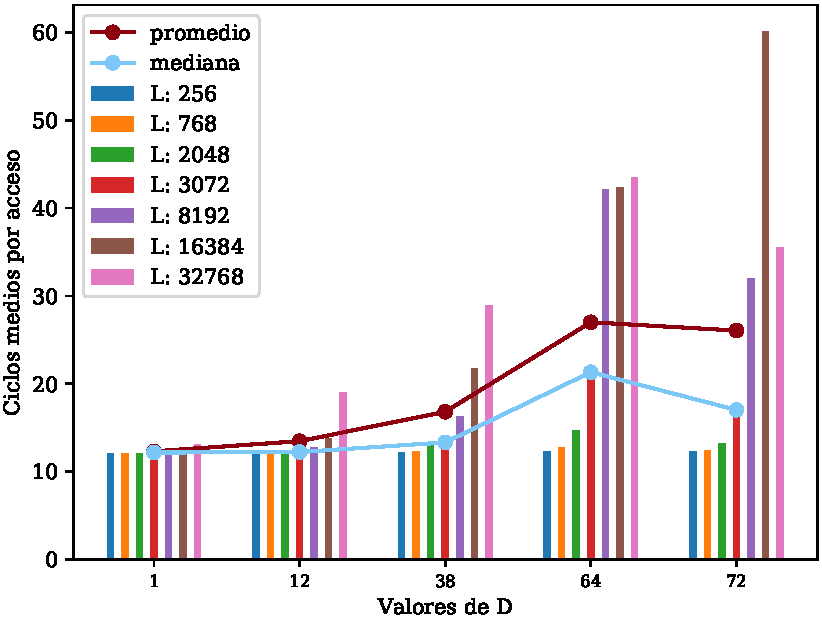
\includegraphics[scale=0.64]{valoresD.pdf}}
\caption{Ciclos medios por acceso a memoria respecto al valor de D. Para cada D se representan los siete posibles valores de L.}
\label{valoresD}
\end{figure}

Como se puede observar, a medida que aumenta el paso entre los valores a los que es necesario acceder, el número de ciclos medios se ve incrementado debido por el motivo comentado previamente.

Por ejemplo, en el caso de \textit{D} = 1, se accede a los datos del array \textit{A[]} de forma secuencial, viéndose claramente en los resultados obtenidos los beneficios del principio de localidad.

Continuando con el caso de \textit{D} = 12, al presentarse en el computador de pruebas líneas caché en las que caben 8 valores \texttt{Double}, cada valor referenciado se encuentra en una línea distinta. En la mayor parte de los casos, estas líneas se dispondrán en memoria de forma consecutiva, mientras que, en otros casos, existirán líneas intermedias que no serán referenciadas; en la Figura \ref{ejemploCache} se puede ver una representación de este suceso. Por lo tanto, el principio de localidad se cumple en menor medida y, para los valores de \textit{L} mayores, la media de ciclos por acceso se ve incrementada.

\begin{figure}[htbp]
\centerline{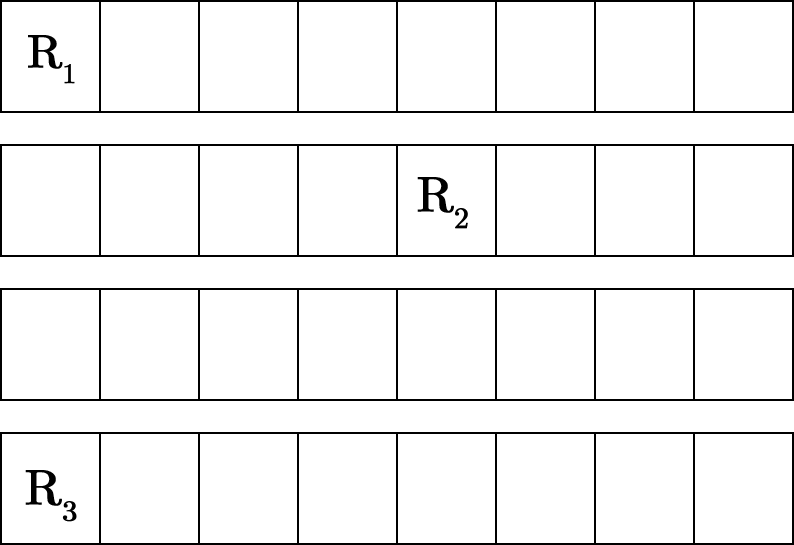
\includegraphics[scale=0.18]{ejemploCache.png}}
\caption{Representación gráfica de omisión de una línea con \textit{D} = 12.}
\label{ejemploCache}
\end{figure}

Observando ahora un caso más pronunciado, con \textit{D} = 72, y considerando el número de valores \texttt{Double} que caben por línea, entre cada una de las referencias siempre quedan ocho líneas a las que no se accede. Esto puede verse claramente reflejado en los valores obtenidos en los correspondientes experimentos.

Finalmente, cabe destacar que lo esperable sería que los experimentos de \textit{D} = 72 resultasen en una mayor cantidad de ciclos medios que en el caso de \textit{D} = 64. Sin embargo, la Figura \ref{valoresD} no muestra este comportamiento, y esto puede ser atribuido a la variabilidad por diversos factores externos a la hora de realizar los experimentos, como que el sistema operativo no sea un entorno completamente aislado, o la asociatividad de las memorias caché.

Tocante a la Figura \ref{valoresL}, se representan los mismos valores de la Figura \ref{valoresD}, solo que invirtiendo la organización entre el eje de abscisas y los conjuntos de barras. El propósito de representación es poder analizar la variabilidad de los ciclos medios desde otro punto de vista, concretamente desde el parámetro \textit{L}.

\begin{figure}[htbp]
\centerline{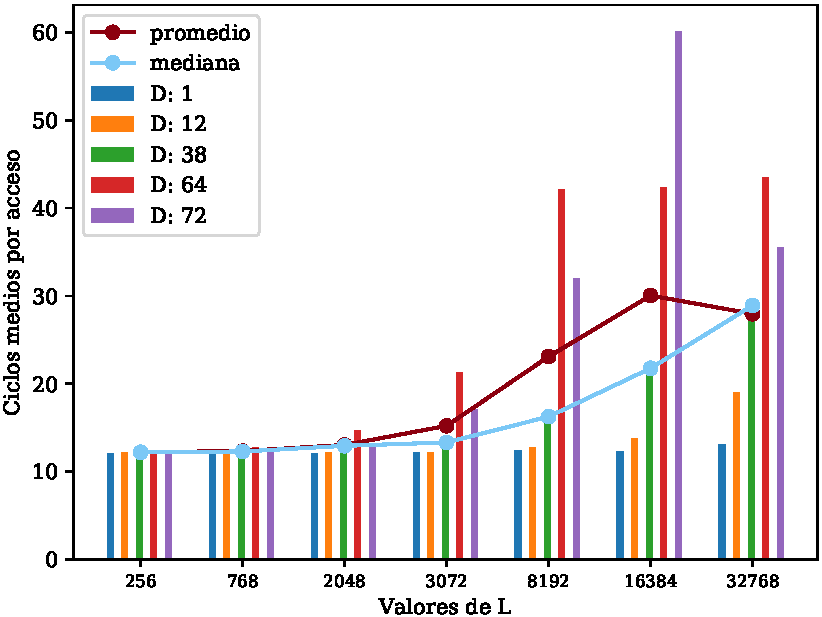
\includegraphics[scale=0.64]{valoresL.pdf}}
\caption{Ciclos medios por acceso a memoria respecto al valor de L. Para cada L se representan los cinco posibles valores de D.}
\label{valoresL}
\end{figure}

Por los motivos descritos anteriormente, a medida que se incrementa el valor del parámetro \textit{L}, también se verán potenciados los efectos producidos a causa de las demás variantes como, por ejemplo, las líneas intermedias sin referenciar.
Consecuentemente, se ve claramente reflejado en la última Figura cómo la tendencia de los ciclos tiende a aumentar a medida que crece \textit{L}.

El argumento de que el valor de \textit{L} potencie los efectos de otros parámetros se ve reforzado, por ejemplo, observando en la Figura \ref{valoresD} los resultados de los experimentos para \textit{D} = 1.

En estos casos, los ciclos medios se ven influenciados por los valores de \textit{L} en mucha menor medida que en los demás casos, puesto que, al encontrar un paso igual a 1, el cumplimiento del principio de localidad se ve favorecido en gran medida. Por lo tanto, una varianza de \textit{L} no supone un cambio significativo en los ciclos medios.

Para realizar una comparativa entre los ciclos medios por acceso a dato y la latencia en el acceso a los diversos niveles de la jerarquía de memoria, se lleva a cabo un benchmark de la suite \textit{LMbench} \cite{lmbenchDescarga}\cite{lmbenchPaper} que permite realizar, entre otras funcionalidades, una estimación de la latencia de la caché de un procesador.

Se realizan las mediciones un total de cuatro veces para una mayor fiabilidad, y los resultados obtenidos se pueden ver representados en la Figura \ref{graficaCache}. Cada una de las regiones planas se corresponde con un nivel de la jerarquía de memoria, y los correspondientes valores se muestran en el Cuadro \ref{latenciasCaches} de un modo más preciso.

\begin{figure}[htbp]
\centerline{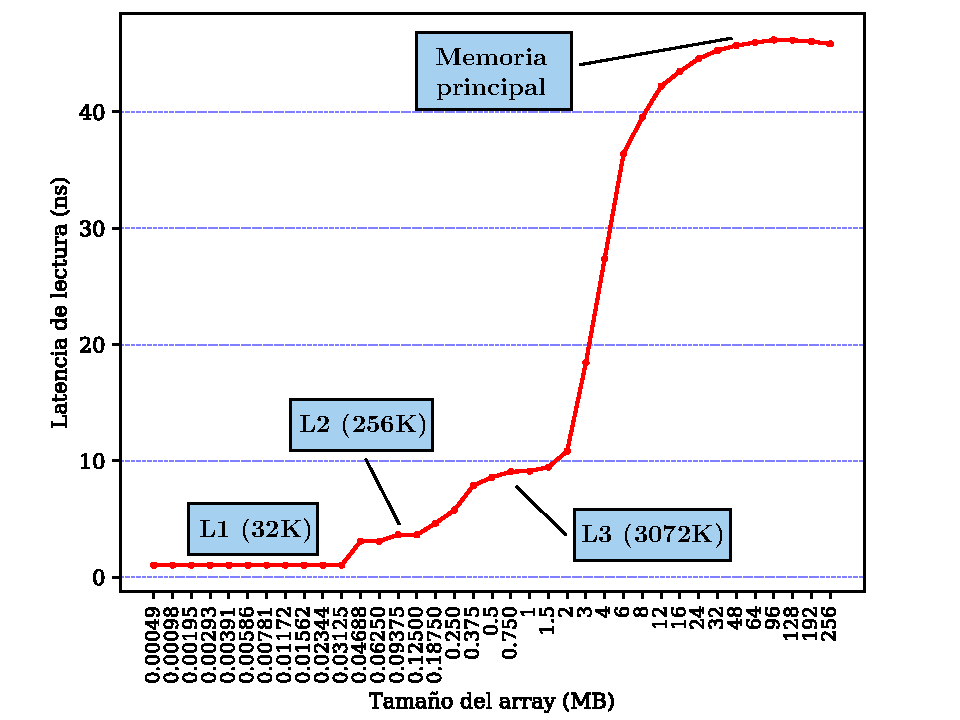
\includegraphics[scale=0.64]{graficaCache.pdf}}
\caption{Tiempos de acceso (ns) obtenidos para parte de la jerarquía de memoria tras la ejecución del benckmark apropiado de la suite \textit{LMbench}.}
\label{graficaCache}
\end{figure}

\begin{table}[htbp]
\caption{Comparativa de niveles de caché de un procesador Intel i3 7100.}
\begin{center}
\begin{tabular}{|>{\columncolor[HTML]{EFEFEF}}c|c|c|c|}
\hline
\textbf{NIVEL} & \cellcolor[HTML]{EFEFEF}\textbf{Capacidad} & \cellcolor[HTML]{EFEFEF}\textbf{Latencia (ns)} & \cellcolor[HTML]{EFEFEF}\textbf{Latencia (ciclos)} \\ \hline
\textbf{L1$^{\mathrm{a}}$}             & 32 KB                                              & 1.0                             & 3.9                                         \\ \hline
\textbf{L2}             & 256 KB                                             & 3.1 - 5.8                             & 12.1 - 22.6                                        \\ \hline
\textbf{L3}             & 3072 KB                                                & 8.5 - 10.9                           & 33.2 - 42.5                                        \\ \hline
\multicolumn{4}{l}{$^{\mathrm{a}}$Tan solo se considera la caché L1 de datos.}
\end{tabular}
\label{latenciasCaches}
\end{center}
\end{table}

Con ello, es posible determinar que, en los mejores casos, los ciclos medios por acceso a dato se sitúan entorno a los mejores valores de la caché L2 del procesador de pruebas. Para verificar que estos datos concuerdan, se analizará por ejemplo el experimento con \textit{D} = 12 y \textit{L} = 3072.

En este caso, siguiendo las fórmulas dispuestas para el cálculo de R y de TC, será necesario reservar e inicializar un total de 36853 bytes. Esta cantidad sobrepasa levemente la capacidad de la caché L1 de datos, por lo cual es coherente que los ciclos medios por acceso a dato se encuentren en torno al mejor rendimiento de la caché L2, siendo necesario considerar para ello que también pueden influir otros factores como la asociatividad de las cachés.

Por otra parte, los valores más altos obtenidos de los experimentos habitúan situarse en torno a las latencias más elevadas de la caché L3. Por ejemplo, con \textit{D} = 72 y \textit{L} = 32768, la cantidad de bytes a reservar e inicializar asciende a más de 2 MB, por lo cual será necesario recurrir a la caché L3.

Es importante considerar el hecho de que estos experimentos se hayan realizado desactivando cualquier tipo de optimización que pueda realizar el compilador. Por ende, si se encarga al compilador la tarea de optimizar el código generado, es posible que, a pesar de trabajar con una cantidad de datos superior a la capacidad de un nivel de la caché, los tiempos promedios obtenidos puedan resultar incluso menores que los esperados.

\subsection{Variabilidad inducida por la técnica de precarga}

\subsubsection{Precarga mediante software}

Como se ha mencionado anteriormente, se emplea el compilador \textit{GCC} empleando la opción \textit{-O0} para evitar que realice optimizaciones. Sin embargo, esta opción ignora además la opción de precarga aunque esta se especifique explícitamente en las opciones de la compilación \cite{noQuiereOptimizar}.

Por lo tanto, para observar la precarga mediante software es necesario especificar, por lo menos, el mínimo nivel de optimización, que es \textit{-O1}. Consecuentemente, además de la precarga, afectarán a los resultados otra serie de optimizaciones asignadas a partir de este nivel.

Para verificar que se están incluyendo las instrucciones de precarga que interpretará el procesador, cada programa es compilado con la opción \textit{-g} para que incluya información de utilidad para depuradores, y este se lee con la herramienta \textit{objdump}, que permite relacionar cada línea en C con sus correspondientes instrucciones en ensamblador.

Con ello, el resultado de compilar el programa deshabilitando explícitamente la precarga sobre arrays se dispone a continuación:

\begin{lstlisting}[style=customasm, basicstyle=\scriptsize, title=Traducción a ensamblador del bucle computacional del programa de pruebas sin incluir la precarga mediante software.]
/***** Pruebas *****/

  // Se registra el contador de la CPU
  start_counter();
  400d83:	b8 00 00 00 00       	mov    $0x0,%eax
  400d88:	e8 e6 fc ff ff       	callq  400a73 <start_counter>
  400d8d:	48 8d 6c 24 40       	lea    0x40(%rsp),%rbp
  400d92:	4c 8d 75 50          	lea    0x50(%rbp),%r14
  400d96:	41 8d 44 24 ff       	lea    -0x1(%r12),%eax
  400d9b:	49 8d 4c 85 04       	lea    0x4(%r13,%rax,4),%rcx
  400da0:	48 89 ee             	mov    % rbp,%rsi
  400da3:	eb 20                	jmp    400dc5 <main+0x253>
  {
      // Se emplean los índices calculados
      for( j = 0, suma = 0; j < R; j++ )
      {
          // Se realiza el acceso a memoria
          suma += valoresA[ e[ j ] ];
  400da5:	48 63 10             	movslq (%rax),%rdx
  400da8:	f2 0f 58 04 d3       	addsd  (%rbx,%rdx,8),%xmm0
  400dad:	48 83 c0 04          	add    $0x4,%rax

  // Se realizan las sumas especificadas
  for( i = 0; i < NUM_S; i++ )
  {
      // Se emplean los índices calculados
      for( j = 0, suma = 0; j < R; j++ )
  400db1:	48 39 c1             	cmp    % rax,%rcx
  400db4:	75 ef                	jne    400da5 <main+0x233>
  400db6:	eb 00                	jmp    400db8 <main+0x246>
          // Se realiza el acceso a memoria
          suma += valoresA[ e[ j ] ];
      }

      // Se almacena la reducción de punto flotante
      valoresS[ i ] = suma;
  400db8:	f2 0f 11 06          	movsd  % xmm0,(%rsi)
  400dbc:	48 83 c6 08          	add    $0x8,%rsi

  // Se registra el contador de la CPU
  start_counter();

  // Se realizan las sumas especificadas
  for( i = 0; i < NUM_S; i++ )
  400dc0:	4c 39 f6             	cmp    % r14,%rsi
  400dc3:	74 12                	je     400dd7 <main+0x265>
  {
      // Se emplean los índices calculados
      for( j = 0, suma = 0; j < R; j++ )
  400dc5:	66 0f ef c0          	pxor   % xmm0,%xmm0
  400dc9:	45 85 e4             	test   % r12d,%r12d
  400dcc:	7e ea                	jle    400db8 <main+0x246>
  400dce:	4c 89 e8             	mov    % r13,%rax
  400dd1:	66 0f ef c0          	pxor   % xmm0,%xmm0
  400dd5:	eb ce                	jmp    400da5 <main+0x233>
      // Se almacena la reducción de punto flotante
      valoresS[ i ] = suma;
  }

  // Se registran los ciclos transcurridos desde el registro del contador
  ck = get_counter();
  400dd7:	b8 00 00 00 00       	mov    $0x0,%eax
  400ddc:	e8 a5 fc ff ff       	callq  400a86 <get_counter>
  400de1:	f2 0f 11 04 24       	movsd  % xmm0,(%rsp)
\end{lstlisting}

Como se puede observar, el bucle computacional no incluye en su traducción a ensamblador ninguna instrucción de precarga. Introduciendo ahora la opción \texttt{fprefetch-loop-arrays}, se genera el siguiente código en ensamblador:

\begin{lstlisting}[style=customasm, basicstyle=\scriptsize, title=Traducción a ensamblador del bucle computacional del programa de pruebas incluyendo la precarga mediante software.]
/***** Pruebas *****/

  // Se registra el contador de la CPU
  start_counter();
  4011f0:	b8 00 00 00 00       	mov    $0x0,%eax
  4011f5:	e8 79 f8 ff ff       	callq  400a73 <start_counter>
  4011fa:	4c 8d 6c 24 50       	lea    0x50(%rsp),%r13
  4011ff:	4d 8d 75 50          	lea    0x50(%r13),%r14
  401203:	4c 89 ef             	mov    % r13,%rdi
  401206:	41 8d 74 24 f1       	lea    -0xf(%r12),%esi
  40120b:	e9 3b 01 00 00       	jmpq   40134b <main+0x7d9>
  {
      // Se emplean los índices calculados
      for( j = 0, suma = 0; j < R; j++ )
      {
          // Se realiza el acceso a memoria
          suma += valoresA[ e[ j ] ];
  401210:	48 63 d0             	movslq % eax,%rdx
  401213:	48 63 14 93          	movslq (%rbx,%rdx,4),%rdx
  401217:	f2 0f 58 44 d5 00    	addsd  0x0(%rbp,%rdx,8),%xmm0

  // Se realizan las sumas especificadas
  for( i = 0; i < NUM_S; i++ )
  {
      // Se emplean los índices calculados
      for( j = 0, suma = 0; j < R; j++ )
  40121d:	83 c0 01             	add    $0x1,%eax
  401220:	41 39 c4             	cmp    % eax,%r12d
  401223:	7f eb                	jg     401210 <main+0x69e>
  401225:	e9 14 01 00 00       	jmpq   40133e <main+0x7cc>
      {
          // Se realiza el acceso a memoria
          suma += valoresA[ e[ j ] ];
  40122a:	48 63 c8             	movslq % eax,%rcx
  40122d:	48 8d 0c 8b          	lea    (%rbx,%rcx,4),%rcx
  401231:	0f 18 49 50          	prefetcht0 0x50(%rcx)
  401235:	48 63 09             	movslq (%rcx),%rcx
  401238:	f2 0f 58 44 cd 00    	addsd  0x0(%rbp,%rcx,8),%xmm0
  40123e:	48 63 ca             	movslq % edx,%rcx
  401241:	48 63 0c 8b          	movslq (%rbx,%rcx,4),%rcx
  401245:	f2 0f 58 44 cd 00    	addsd  0x0(%rbp,%rcx,8),%xmm0
  40124b:	8d 48 02             	lea    0x2(%rax),%ecx
  40124e:	48 63 c9             	movslq % ecx,%rcx
  401251:	48 63 0c 8b          	movslq (%rbx,%rcx,4),%rcx
  401255:	f2 0f 58 44 cd 00    	addsd  0x0(%rbp,%rcx,8),%xmm0
  40125b:	8d 48 03             	lea    0x3(%rax),%ecx
  40125e:	48 63 c9             	movslq % ecx,%rcx
  401261:	48 63 0c 8b          	movslq (%rbx,%rcx,4),%rcx
  401265:	f2 0f 58 44 cd 00    	addsd  0x0(%rbp,%rcx,8),%xmm0
  40126b:	8d 48 04             	lea    0x4(%rax),%ecx
  40126e:	48 63 c9             	movslq % ecx,%rcx
  401271:	48 63 0c 8b          	movslq (%rbx,%rcx,4),%rcx
  401275:	f2 0f 58 44 cd 00    	addsd  0x0(%rbp,%rcx,8),%xmm0
  40127b:	8d 48 05             	lea    0x5(%rax),%ecx
  40127e:	48 63 c9             	movslq % ecx,%rcx
  401281:	48 63 0c 8b          	movslq (%rbx,%rcx,4),%rcx
  401285:	f2 0f 58 44 cd 00    	addsd  0x0(%rbp,%rcx,8),%xmm0
  40128b:	8d 48 06             	lea    0x6(%rax),%ecx
  40128e:	48 63 c9             	movslq % ecx,%rcx
  401291:	48 63 0c 8b          	movslq (%rbx,%rcx,4),%rcx
  401295:	f2 0f 58 44 cd 00    	addsd  0x0(%rbp,%rcx,8),%xmm0
  40129b:	8d 48 07             	lea    0x7(%rax),%ecx
  40129e:	48 63 c9             	movslq % ecx,%rcx
  4012a1:	48 63 0c 8b          	movslq (%rbx,%rcx,4),%rcx
  4012a5:	f2 0f 58 44 cd 00    	addsd  0x0(%rbp,%rcx,8),%xmm0
  4012ab:	8d 48 08             	lea    0x8(%rax),%ecx
  4012ae:	48 63 c9             	movslq % ecx,%rcx
  4012b1:	48 63 0c 8b          	movslq (%rbx,%rcx,4),%rcx
  4012b5:	f2 0f 58 44 cd 00    	addsd  0x0(%rbp,%rcx,8),%xmm0
  4012bb:	8d 48 09             	lea    0x9(%rax),%ecx
  4012be:	48 63 c9             	movslq % ecx,%rcx
  4012c1:	48 63 0c 8b          	movslq (%rbx,%rcx,4),%rcx
  4012c5:	f2 0f 58 44 cd 00    	addsd  0x0(%rbp,%rcx,8),%xmm0
  4012cb:	8d 48 0a             	lea    0xa(%rax),%ecx
  4012ce:	48 63 c9             	movslq % ecx,%rcx
  4012d1:	48 63 0c 8b          	movslq (%rbx,%rcx,4),%rcx
  4012d5:	f2 0f 58 44 cd 00    	addsd  0x0(%rbp,%rcx,8),%xmm0
  4012db:	8d 48 0b             	lea    0xb(%rax),%ecx
  4012de:	48 63 c9             	movslq % ecx,%rcx
  4012e1:	48 63 0c 8b          	movslq (%rbx,%rcx,4),%rcx
  4012e5:	f2 0f 58 44 cd 00    	addsd  0x0(%rbp,%rcx,8),%xmm0
  4012eb:	8d 48 0c             	lea    0xc(%rax),%ecx
  4012ee:	48 63 c9             	movslq % ecx,%rcx
  4012f1:	48 63 0c 8b          	movslq (%rbx,%rcx,4),%rcx
  4012f5:	f2 0f 58 44 cd 00    	addsd  0x0(%rbp,%rcx,8),%xmm0
  4012fb:	8d 48 0d             	lea    0xd(%rax),%ecx
  4012fe:	48 63 c9             	movslq % ecx,%rcx
  401301:	48 63 0c 8b          	movslq (%rbx,%rcx,4),%rcx
  401305:	f2 0f 58 44 cd 00    	addsd  0x0(%rbp,%rcx,8),%xmm0
  40130b:	8d 48 0e             	lea    0xe(%rax),%ecx
  40130e:	48 63 c9             	movslq % ecx,%rcx
  401311:	48 63 0c 8b          	movslq (%rbx,%rcx,4),%rcx
  401315:	f2 0f 58 44 cd 00    	addsd  0x0(%rbp,%rcx,8),%xmm0
  40131b:	8d 48 0f             	lea    0xf(%rax),%ecx
  40131e:	48 63 c9             	movslq % ecx,%rcx
  401321:	48 63 0c 8b          	movslq (%rbx,%rcx,4),%rcx
  401325:	f2 0f 58 44 cd 00    	addsd  0x0(%rbp,%rcx,8),%xmm0
  40132b:	83 c0 10             	add    $0x10,%eax
  40132e:	83 c2 10             	add    $0x10,%edx
  401331:	39 d6                	cmp    %edx,%esi
  401333:	0f 8f f1 fe ff ff    	jg     40122a <main+0x6b8>
  401339:	e9 d2 fe ff ff       	jmpq   401210 <main+0x69e>
      }

      // Se almacena la reducción de punto flotante
      valoresS[ i ] = suma;
  40133e:	f2 0f 11 07          	movsd  % xmm0,(%rdi)
  401342:	48 83 c7 08          	add    $0x8,%rdi

  // Se registra el contador de la CPU
  start_counter();

  // Se realizan las sumas especificadas
  for( i = 0; i < NUM_S; i++ )
  401346:	4c 39 f7             	cmp    % r14,%rdi
  401349:	74 37                	je     401382 <main+0x810>
  {
      // Se emplean los índices calculados
      for( j = 0, suma = 0; j < R; j++ )
  40134b:	66 0f ef c0          	pxor   % xmm0,%xmm0
  40134f:	45 85 e4             	test   % r12d,%r12d
  401352:	7e ea                	jle    40133e <main+0x7cc>
  401354:	83 fe 01             	cmp    $0x1,%esi
  401357:	7e 1b                	jle    401374 <main+0x802>
  401359:	ba 01 00 00 00       	mov    $0x1,%edx
  40135e:	b8 00 00 00 00       	mov    $0x0,%eax
  401363:	66 0f ef c0          	pxor   % xmm0,%xmm0
  401367:	41 81 fc 0f 00 00 80 	cmp    $0x8000000f,%r12d
  40136e:	0f 8d b6 fe ff ff    	jge    40122a <main+0x6b8>
  401374:	b8 00 00 00 00       	mov    $0x0,%eax
  401379:	66 0f ef c0          	pxor   % xmm0,%xmm0
  40137d:	e9 8e fe ff ff       	jmpq   401210 <main+0x69e>
      // Se almacena la reducción de punto flotante
      valoresS[ i ] = suma;
  }

  // Se registran los ciclos transcurridos desde el registro del contador
  ck = get_counter();
  401382:	b8 00 00 00 00       	mov    $0x0,%eax
  401387:	e8 fa f6 ff ff       	callq  400a86 <get_counter>
  40138c:	f2 0f 11 04 24       	movsd  % xmm0,(%rsp)
\end{lstlisting}

Ahora sí se introducen en el programa instrucciones de precarga, concretamente en tres situaciones: en la generación de los valores del array \textit{A[]}, en la generación de los índices contenidos en el array \textit{e[]}, y en el bucle computacional. Tan solo se representa este último caso por cuestiones de espacio.

Cabe destacar además que en el primer y último caso se replica el código correspondiente a cada línea de C para ejecutarla un total de 16 veces de forma secuencial. Además, estas líneas no cuentan con una única traducción en código ensamblador.

Antes de continuar, debe considerarse que en el bucle computacional se efectúa un acceso a un array de forma indirecta, pero tan sólo se incluye una instrucción de precarga en cada iteración. Por lo tanto, el compilador puede haber decidido emplear esta técnica o bien sobre \textit{A[]}, o bien sobre \textit{e[]}.

Para aclarar esta cuestión, se modifica ligeramente el código del programa. Ahora, se obtiene en primer lugar un índice accediendo a \textit{e[]} y, tras ello, se accede a la posición de \textit{A[]} apropiada. El resultado de la compilación es el siguiente:

\begin{lstlisting}[style=customasm, basicstyle=\scriptsize, title=Fragmento de la traducción a ensamblador del bucle computacional del programa de pruebas incluyendo la precarga mediante software.]
          // Se realiza el acceso a memoria
          indice = e[ j ];
  40122a:	48 63 c8             	movslq % eax,%rcx
  40122d:	48 8d 0c 8b          	lea    (%rbx,%rcx,4),%rcx
  401231:	0f 18 49 50          	prefetcht0 0x50(%rcx)
          suma += valoresA[ indice ];
  401235:	48 63 09             	movslq (%rcx),%rcx
  401238:	f2 0f 58 44 cd 00    	addsd  0x0(%rbp,%rcx,8),%xmm0
\end{lstlisting}

De este modo sí es posible observar cómo la instrucción de precarga generada corresponde a la línea de C en la que se referencia un valor de \textit{e[]}, por lo cual se puede concluir que la precarga no se realiza sobre el array \textit{A[]}. Consecuentemente, la precarga mediante software no debería suponer una notable diferencia en términos de rendimiento, puesto que simplemente se precargan elementos a los que se accede de por sí de forma secuencial y, por lo tanto, el principio de localidad beneficiará claramente la ejecución.

Sin embargo, es de interés considerar la ''réplica`` de instrucciones en ensamblador llevada a cabo así como la disponibilidad de diversas implementaciones de algunas líneas de C. Como se puede observar en el código dispuesto anteriormente, en cada iteración de una versión del bucle computacional se realizan, aparentemente, 16 sumas en lugar de una única. Además, la instrucción de precarga se sitúa al inicio de este mismo. Sabiendo que la precarga se efectúa sobre los elementos de \textit{e[]}, que son de tipo \texttt{int} (4 bytes), y que una línea del computador de pruebas contiene 64 bytes, en cada una de ellas se pueden almacenar 16 valores de \textit{e[]}.

Por todo ello, es probable que el compilador decida realizar la siguiente optimización: si es posible, se realizan 16 iteraciones originales del bucle en una única, indicando al inicio de esta última que se traiga la siguiente línea de elementos de \textit{e[]} que podrán ser empleados en la siguiente iteración. De este modo, mientras se emplean los 16 elementos disponibles de \textit{e[]}, los siguientes 16 son traídos simultáneamente evitando, si es posible, que se produzca un fallo de caché al inicio de la próxima iteración. En caso de que simplemente sea imposible realizar 16 sumas consecutivas, se emplea una versión alternativa en ensamblador del bucle computacional, realizando las sumas de una en una al igual que en el código original en C.

Si esta es realmente la optimización llevada a cabo por el compilador, quizá sí sea posible percibir una mejora sobre la velocidad de ejecución como consecuencia de la precarga, al poder evitar que se produzca un fallo de caché por tratar de leer un índice que no se encuentre en ella.

Finalmente, cabe destacar que se ha tratado de forzar, sin éxito, que el compilador efectúe la precarga sobre el array \textit{A[]}, dado que los índices almacenados en \textit{e[]} se encuentran equiespaciados, y quizá sería capaz de detectar dicho patrón en esos accesos a memoria. Las pruebas realizadas son las siguientes:

\begin{itemize}
    \item Eliminar el bucle correspondiente a las diez reducciones de punto flotante, realizándose tan solo una con el objetivo de reducir la complejidad del código de cara al compilador, puesto que se encontraba con dos bucles \texttt{for} anidados.
    \item En lugar de obtener los índices a partir del array \textit{e[]}, se accede a un valor de \textit{A[]} directamente en función del número de iteración, del mismo modo en que los índices son generados, resultando en \texttt{suma += valoresA[ j * D ]}.
    \item Las dos anteriores pruebas conjuntas.
    \item Emplear el compilador Clang para comprobar su política a la hora de efectuar las optimizaciones.
\end{itemize}

A continuación, se pueden observar en la Figura \ref{NoPrecargaSoftware} los ciclos medios por acceso obtenidos sin realizar la precarga de los elementos de \textit{e[]}.

\begin{figure}[htbp]
\centerline{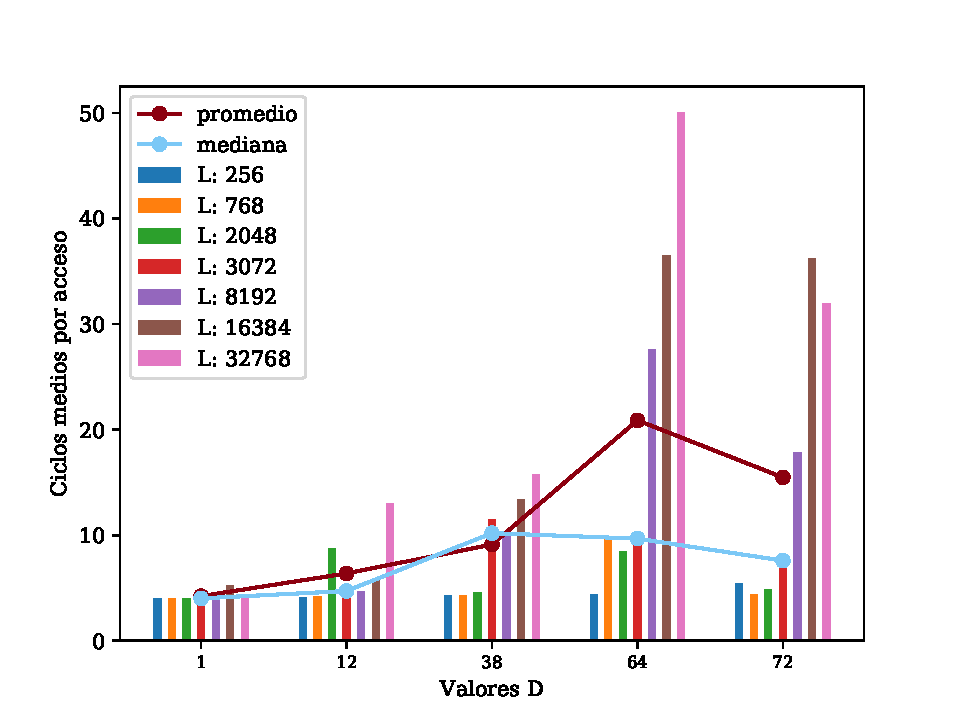
\includegraphics[scale=0.64]{NoPrecargaSoftware.pdf}}
\caption{Ciclos medios por acceso a memoria respecto al valor de D sin emplear la precarga mediante software (nivel 1 de optimización).}
\label{NoPrecargaSoftware}
\end{figure}

Y, para poder estudiar la eficiencia a la hora de precargar los índices, se comparará la Figura anterior con la Figura \ref{precargaSoftware}, en la que se muestran los ciclos medios obtenidos empleando la precarga sobre los índices contenidos en \textit{e[]}.

\begin{figure}[htbp]
\centerline{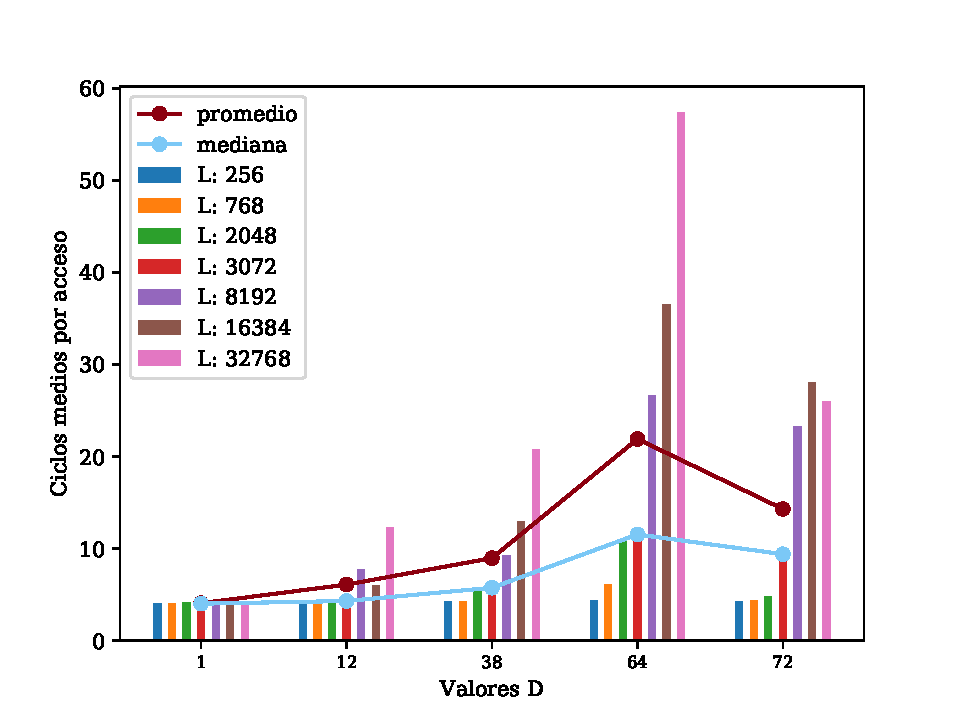
\includegraphics[scale=0.64]{PrecargaSoftware.pdf}}
\caption{Ciclos medios por acceso a memoria respecto al valor de D empleando la precarga mediante software (nivel 1 de optimización).}
\label{precargaSoftware}
\end{figure}

Estas figuras muestran que, el hecho de realizar la precarga por software o no, no supone una variabilidad relevante de los ciclos medios por acceso.

De todos modos, puede observarse que la precarga puede afectar a los valores más pequeños de \textit{D} y de \textit{L}, como pueden ser \textit{D} = 1 o \textit{D} = 38, y \textit{L} = 256 o \textit{L} = 2048. En estos casos, es posible que los ciclos medios sí se puedan ven incrementados en la Figura \ref{NoPrecargaSoftware} respecto a la Figura \ref{precargaSoftware}.

Este puede suceder por las siguientes cuestiones:

\begin{itemize}
    \item Si un experimento presenta un número de ciclos medios reducido, como por ejemplo los casos de \textit{D} = 1, una pequeña variación en el rendimiento a la hora de la ejecución se hará notar en mayor medida que en un experimento como el de \textit{D} = 64 y \textit{L} = 32768, en que se dan valores mucho más elevados.
    \item Es relevante además el tamaño del experimento, es decir, el número de elementos a inicializar y a leer, puesto que la precarga por software se puede hacer notar en mayor medida en casos pequeños respecto a la precarga por hardware, la cual necesita identificar patrones en accesos a datos para funcionar correctamente. Consecuentemente, es posible que los experimentos de mayor envergadura se vean influenciados de una manera importante por la precarga mediante hardware, y por ende la precarga por software no varíe tanto los resultados.
\end{itemize}

\subsubsection{Precarga mediante hardware}

Como se explicó anteriormente, la precarga por hardware es inherente al procesador de pruebas, por lo que simplemente es posible tratar de reducir su efectividad, en lugar de desactivarla como en el caso de la precarga mediante software.

Para ello, se realiza la modificación especificada anteriormente, y el segmento del programa de pruebas en donde se generan los índices resulta del siguiente modo:

\begin{lstlisting}[style=CStyle, title=Programa de pruebas en el que se trata de evitar la precarga mediante hardware.]
ENTORNO = 3

for( i = 0; i < R; i++ )
{
    // Se consideran el número de posición y el paso// dado junto a un entero aleatorio entre [0,   // ENTORNO]
    e[ i ] = i * D + rand()% ENTORNO;
}
\end{lstlisting}

El programa es compilado con la opción \textit{-O0}, dado que ya que no es necesario forzar una optimización mediante software. Se pueden observar los resultados obtenidos en la Figura \ref{precargaHardware}. Comparándola con la Figura \ref{valoresD}, la progresión de los ciclos medios (promedio y mediana) a medida que crece el valor de \textit{D} se mantiene prácticamente igual en la mayor parte de los casos.

\begin{figure}[htbp]
\centerline{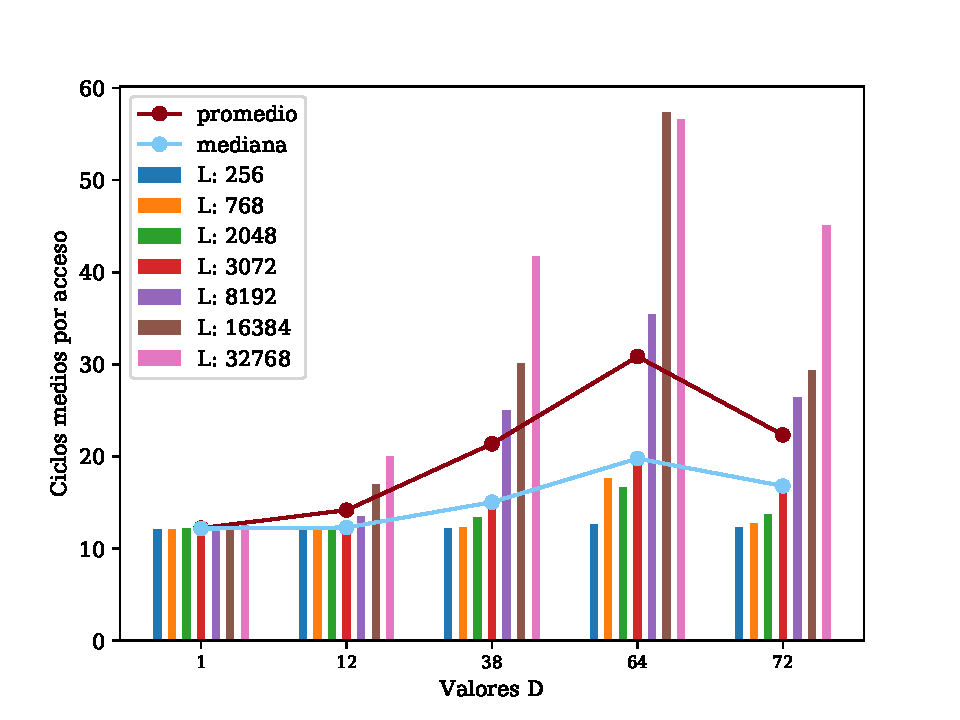
\includegraphics[scale=0.64]{QuemarHardware.pdf}}
\caption{Ciclos medios por acceso a memoria respecto al valor de D tratando de evitar la precarga mediante hardware.}
\label{precargaHardware}
\end{figure}

Sin embargo, considerando el tamaño total de los experimentos, es decir, la combinación de \textit{D} y \textit{L}, se puede observar que en los casos intermedios sí se produce un leve incremento de los ciclos medios respecto a la Figura \ref{valoresD}. Esto se puede ver reflejado en experimentos como \textit{D} = 12 y \textit{L} = 16384, \textit{D} = 38 y \textit{L} = 8192, o \textit{D} = 64 y \textit{L} = 768.

Esto puede ser debido a que, para tamaños pequeños, la efectividad del principio de localidad evita que la variabilidad de la precarga por hardware afecte de forma importante a los resultados. Por otra parte, para tamaños grandes, los resultados de los experimentos muestran que la ejecución se ve notablemente perjudicada debido a que los parámetros dados no favorecen que se cumpla el principio de localidad, y por lo tanto la pequeña variabilidad en los intentos de burlar la precarga mediante hardware no se hace notar.

Finalmente, cabe destacar que se producen dos picos en los dos últimos experimentos con \textit{D} = 64, que simplemente pueden deberse a otros factores. Sucede algo similar con el pico de la Figura \ref{valoresD} para \textit{D} = 72 y \textit{L} = 16384.

\section{Conclusiones de los experimentos} \label{resumenExperimentos}

A partir de los experimentos realizados, se puede extraer una serie de conclusiones acerca de la influencia del principio de localidad en la ejecución de un programa que depende en gran medida del acceso a datos, y sobre la efectividad de las técnicas de precarga disponibles para el procesador de pruebas.

Comenzando con el principio de localidad, se concluye que, a medida que los datos se encuentran más distanciados entre sí, el número de ciclos medio por acceso a dato se ve incrementado en función de ello. Esto se debe a que se cumple en menor medida el principio de localidad y, por lo tanto, el rendimiento en la ejecución se ve claramente degradado.

A mayores, también se puede observar que estos resultados se ven influenciados por el número de líneas caché (parámetro \textit{L}) a las que se debe acceder; es decir, el principal determinante del tamaño de un experimento. Por ejemplo, en un caso en el que el principio de localidad apenas se cumpla, las consecuencias de ello se harán notar en mayor medida al realizarse un mayor número de accesos.

Tocante a las implementaciones disponibles para la precarga, se pueden extraer dos conclusiones.

En cuanto a la precarga mediante \textit{software}, esta no condiciona de forma notable el resultado de los experimentos.

Además, es necesario tener en cuenta el compilador empleado, dado que se relega a este la tarea de optimizar el código generado para incluir este tipo de precarga. El compilador debería realizarlo de una forma óptima para no perjudicar el rendimiento del programa compilado, puesto que la inclusión de la precarga resulta en un mayor número de instrucciones en ensamblador, y además todas ellas implican la carga de datos. Por lo tanto, un empleo incorrecto de estas instrucciones supondría una mayor carga sobre el procesador y el desaprovechamiento de parte de la memoria caché.

Por otro lado, la precarga mediante \textit{hardware} es inherente al procesador empleado y, por lo tanto, no es posible que el programador la deshabilite para observar su influencia en el rendimiento del programa. Por lo tanto, tan solo se ha podido intentar evitarla distorsionando los patrones de acceso a datos, y tan solo se han podido observar unos pocos experimentos en los que se vean reflejados sus beneficios, siendo imposible extraer una conclusión global.

\begin{thebibliography}{00}
\bibitem{procesador} Intel Corporation, ``Intel Core i3-7100 Processor (3M Cache, 3.90 GHz) Product Especification'' [en línea]. Disponible en: \url{https://ark.intel.com/content/www/us/en/ark/products/97455/intel-core-i3-7100-processor-3m-cache-3-90-ghz.html} [fecha de consulta: 24/02/2019].
\bibitem{lmbenchDescarga} Larry McVoy, Carl Staelin, ``LMbench - Tools for Performance Analysis'' [en línea]. Disponible en: \url{http://lmbench.sourceforge.net/} [fecha de consulta: 28/02/2019].
\bibitem{lmbenchPaper} Larry McVoy, Carl Staelin, ``lmbench: Portable Tools for Performance Analysis'' [en línea]. Disponible en: \url{https://www.usenix.org/legacy/publications/library/proceedings/sd96/full_papers/mcvoy.pdf} [fecha de consulta: 28/02/2019].
\bibitem{precargas} Intel Corporation, ``Intel® 64 and IA-32 Architectures Software Developer’s Manual Combined Volumes: 1, 2A, 2B, 2C, 2D, 3A, 3B, 3C, 3D, and 4 | Intel® Software'' [en línea]. Disponible en: \url{https://software.intel.com/en-us/download/intel-64-and-ia-32-architectures-sdm-combined-volumes-1-2a-2b-2c-2d-3a-3b-3c-3d-and-4} [fecha de consulta: 03/03/2019].
\bibitem{noQuiereOptimizar} GCC project, ``John (Eljay) Love-Je - RE: Undocumented optimization flag, switched by O1'' [en línea]. Disponible en: \url{https://gcc.gnu.org/ml/gcc-help/2007-11/msg00214.html} [fecha de consulta: 03/03/2019].
\bibitem{hennessy} John L. Hennessy, y David A. Patterson, ``Computer Architecture: A Quantitative Approach,'' Quinta Edición, Morgan Kaufmann, 2011.
\end{thebibliography}

\end{document}
